\documentclass[addpoints, 12pt]{exam}%, answers]
\usepackage[utf8]{inputenc}
\usepackage[T1]{fontenc}

\usepackage{lmodern}
\usepackage{arydshln}
\usepackage[margin=2cm]{geometry}

\usepackage{enumitem}
\usepackage{multicol}

\usepackage{enumerate}
\usepackage{breqn}
\usepackage{parskip}

\usepackage{amsmath, amsthm, amsfonts, amssymb}
\usepackage{graphicx}
\usepackage{tikz}
\usetikzlibrary{arrows,calc,patterns}
\usepackage{pgfplots}
\pgfplotsset{compat=newest}
\usepackage{url}
\usepackage{multicol}
\usepackage{thmtools}

\usepackage{caption}
\usepackage{subcaption}

\usepackage{pifont}

% MATH commands
\newcommand{\bC}{\mathbb{C}}
\newcommand{\bR}{\mathbb{R}}
\newcommand{\bN}{\mathbb{N}}
\newcommand{\bZ}{\mathbb{Z}}
\newcommand{\bT}{\mathbb{T}}
\newcommand{\bD}{\mathbb{D}}

\DeclareMathOperator{\dom}{dom}

\newcommand{\spc}{\vspace*{0.5cm}}
\CorrectChoiceEmphasis{\color{red}}

\begin{document}
\noindent \hrulefill \\
	MATH-241 Calculus I \hfill Created by Rukiyah Walker\\
	Homework 11 \hfill Spring 2023\\ \vspace*{-1cm}
 
	\noindent\hrulefill

\qformat{\rule{0.3\textwidth}{.4pt} \begin{large}{\textsc{Question}} \thequestion \end{large} \hspace*{0.2cm} \hrulefill \hspace*{0.1cm} \textbf{(\totalpoints\hspace*{0.1cm} pts)}}

\begin{questions}

\vspace*{0.5cm}

\question[1]

What is Newton's Method used for?

\begin{multicols}{2}
\begin{choices}
\choice Finding the derivative of a polynomial of degree 5 or higher.
\choice To show that a derivative exists.
\choice To show that $\lim_{n \to \infty} x_n$ exists.
\CorrectChoice Finding an approximation of the root(s) of a function.
\end{choices}  
\end{multicols}

\question[1]

When might Newton's Method fail?

\begin{multicols}{2}
\begin{choices}
\CorrectChoice When $f'(x)$ is close to 0.
\choice When $f(x) = f'(x)$.
\choice When $\lim_{x \to \infty} f(x) = 0$.
\choice When $x_{n+1} = x_n$.
\end{choices}
\end{multicols}

\question[1]

How can you still use Newton's Method after it fails?

\begin{multicols}{2}
\begin{choices}
\choice Set $f(x) = 0$.
\choice Use a different method.
\CorrectChoice Choose a better initial approximation, $x_1$.
\choice Set $x_{n+1} = x_n$.
\end{choices} 
\end{multicols}

\question[1]

Newton's Method says the next approximation is given by $x_{n+1} = x_n - \frac{f(x_n)}{f'(x_n)}$, where $x_n$ is the $n$th approximation and $f'(x_n) \neq 0$. 
If the numbers $x_n$ become closer and closer to some number $r$ as $n$ becomes large, we say that the sequence converges to $r$. What does this mean in terms of limits?

\begin{multicols}{2}
\begin{choices}
\choice $\lim_{x \to \infty} n = r$
\CorrectChoice $\lim_{n \to \infty} x_n = r$ 
\choice $\lim_{x \to \infty} x = r$
\choice $\lim_{r \to \infty} x_n = \infty$
\end{choices}  
\end{multicols}


\question[1]

A function $F$ is called an antiderivative of $f$ on an interval $I$ if $F'(x) = f(x)$ for all $x$ in $I$. What does this mean?

\begin{multicols}{2}
\begin{choices}
\CorrectChoice $F$ is a function whose derivative is equal to the original function $f$.
\choice $\lim_{x \to \infty} F'(x) = f(x)$
\choice There exists only one antiderivative for $f(x)$.
\choice $\lim_{x \to \infty} f(x) = F'(x)$
\end{choices}  
\end{multicols}

\newpage

\question[1]

What is the general antiderivative of $f(x) = x^n$?

\begin{multicols}{2}
\begin{choices}
\choice $F(x) = \frac{x^{n+1}}{n+1}$
\choice $F(x) = \frac{(n+1)x}{n+1} + C$
\CorrectChoice $F(x) = \frac{x^{n+1}}{n+1} + C$
\choice $F(x) = \frac{(n+1)x}{n+1}$
\end{choices} 
\end{multicols}

\spc

\question[1]

Which of the following is NOT an example of an antiderivative of  the function $f(x) = x^2 + x$?

\begin{multicols}{2}
\begin{choices}
\choice $F(x) = \frac{x^3}{3} + \frac{x^2}{2} + C$
\choice $F(x) = \frac{x^3}{3} + \frac{x^2}{2} + 2$
\choice $F(x) = \frac{x^3}{3} + \frac{x^2}{2} + 100$
\CorrectChoice $F(x) = \frac{x^3}{3} + \frac{x^2}{2} + 2x$
\end{choices}
\end{multicols}

\spc

\question[1]

Find the antiderivative of $f(x) = x^2 + 2x$ given $F(0) = 1$.

\begin{multicols}{2}
\begin{choices}
\choice $F(x) = \frac{x^3}{3} + x^2$
\CorrectChoice $F(x) = \frac{x^3}{3} + x^2 +1$.
\choice $F(x) = \frac{x^3}{3} + \frac{x}{2}$
\choice $F(x) = 1$
\end{choices}
\end{multicols}

\spc

\question[1]

Find the antiderivative of $f(x) = \frac{2x^3 + \sqrt{x}}{x}$ given $F(1) = 2$.

\begin{multicols}{2}
\begin{choices}
\CorrectChoice $F(x) = \frac{2}{3}x^3 + 2x^{1/2} - \frac{8}{3}$
\choice $F(x) = \frac{8}{3}$
\choice $F(x) = \frac{x^3}{3} + 2x^{1/2}$
\choice $F(x) = \frac{2}{3}x^3 + 2x^{1/2}$
\end{choices}
\end{multicols}

\spc

\question[1]

How can we approximate the area of the region S which lies under the curve $y = x^2$?

\begin{minipage}{0.5\textwidth}
\begin{choices}
\choice Take the derivative of $y = x^2$. \vspace*{10pt}
\choice Use the height of the function $(h)$ and length of the interval $(l)$, then $A = hl$. \vspace*{10pt}
\CorrectChoice Divide the interval into a bunch of subintervals (rectangles) of equal length then take the sum of the areas of the rectangles. \vspace*{10pt}
\choice Use newton's method. \vspace*{10pt}
\end{choices}
\end{minipage}
\hspace*{1cm}
\begin{minipage}{0.35\textwidth}
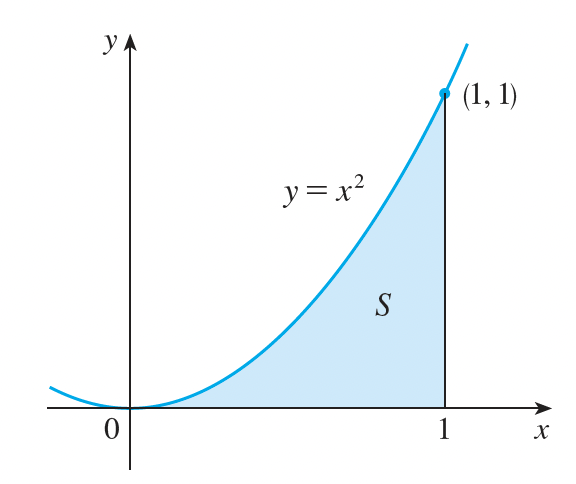
\includegraphics[width=1\textwidth]{Homework11-graph.png}
\end{minipage}



\end{questions}
\end{document}